\documentclass[11pt,letterpaper]{article}
\usepackage[lmargin=1in,rmargin=1in,tmargin=1in,bmargin=1in]{geometry}
\usepackage{../style/homework}
\usepackage{../style/commands}
\setbool{quotetype}{true} % True: Side; False: Under
\setbool{hideans}{false} % Student: True; Instructor: False

% -------------------
% Content
% -------------------
\begin{document}

\homework{9: Due 10/24}{You're a good boy, Jeff.}{Catherie Dahmer, \par Dahmer - Monster: \par The Jeffrey Dahmer Story}

% Problem 1
\problem{10} Let $f(x)$ be a function such that $f^{-1}(x)$ exists. A partial table of values for $f(x)$ is given below: \par
	\begin{table}[!ht]
	\centering
	\begin{tabular}{|r||c|c|c|c|c|} \hline 
	$x$ & $1$ & $2$ & $3$ & $4$ & $5$ \\ \hline
	$f(x)$ & $5$ & $7$ & $0$ & $9$ & $3$ \\ \hline
	\end{tabular}
	\end{table}
Based on the table above (or your knowledge of functions and inverses), find the following:
	\begin{enumerate}[(a)]
	\item $f(3)= 0$
	\item $f^{-1}(3)= 5$
	\item $f(4)= 9$
	\item $f^{-1}(9)= 4$
	\item $f(f^{-1}(5))= f(1)= 5$
	\item $f^{-1} \big( f(2) \big)= f^{-1}(7)= 2$
	\item $f^{-1} \big( f(-8) \big)= -8$
	\item $f \big( f^{-1}(10) \big)= 10$
	\end{enumerate}



\newpage



% Problem 2
\problem{10} Let $f(x)= \frac{1}{4} (x - 3)$. Assume that $f^{-1}(x)$ exists. 
	\begin{enumerate}[(a)]
	\item Find $f(15)$. 
	\item Use (a) to explain why $f^{-1}(3)= 15$. 
	\item Solve the equation given by $f(x)= 11$.
	\item Use (c) to explain why $f^{-1}(11)= 47$. 
	\end{enumerate} \pspace

\sol 
\begin{enumerate}[(a)]
\item We have\dots
	\[
	f(15)= \frac{1}{4} \, (15 - 3)= \frac{1}{4} \cdot 12= 3
	\] \pspace

\item We know from (a) that $f(15)= 3$. But then we must have $f^{-1}(3)= 15$. \pspace

\item We have\dots
	\[
	\begin{aligned}
	f(x)&= 11 \\[0.3cm]
	\frac{1}{4}\, (x - 3)&= 11 \\[0.3cm]
	x - 3&= 44 \\[0.3cm]
	x&= 47
	\end{aligned}
	\] \pspace

\item We know from (c) that if $f(x)= 11$, then $x= 47$. But then $f(47)= 11$. This shows that $f^{-1}(11)= 47$. 
\end{enumerate}



\newpage



% Problem 3
\problem{10} A graph of a relation $f(x)$ is shown below:
	\[
	\fbox{
	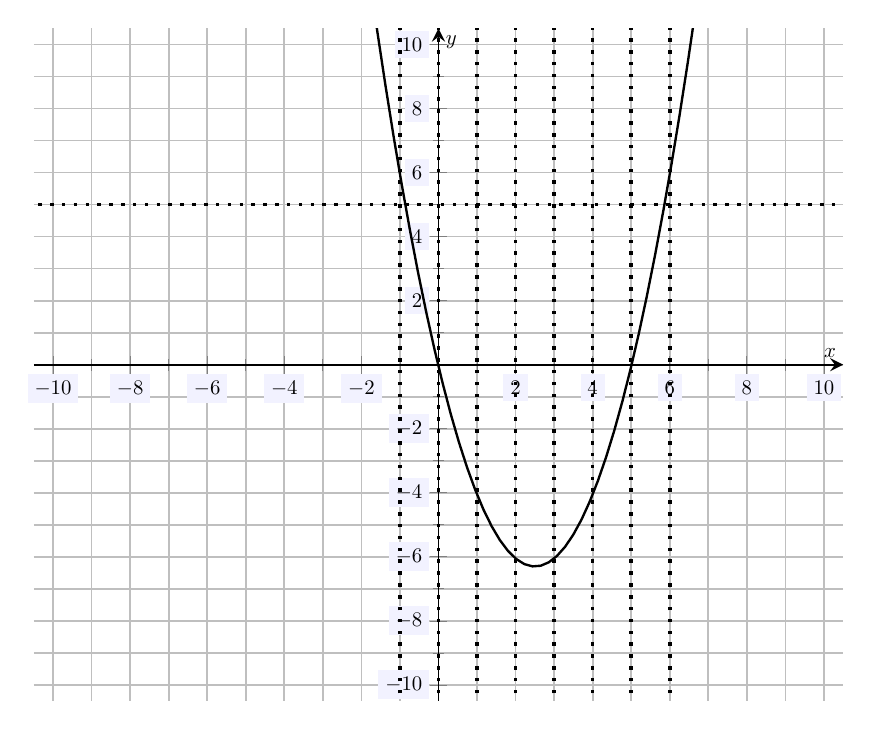
\begin{tikzpicture}[scale=1.5,every node/.style={scale=0.5}]
	\begin{axis}[
	grid=both,
	axis lines=middle,
	ticklabel style={fill=blue!5!white},
	xmin= -10.5, xmax=10.5,
	ymin= -10.5, ymax=10.5,
	xtick={-10,-8,-6,-4,-2,0,2,4,6,8,10},
	ytick={-10,-8,-6,-4,-2,0,2,4,6,8,10},
	minor tick = {-10,-9,...,10},
	xlabel=\(x\),ylabel=\(y\),
	]
	\addplot[line width= 0.02cm,samples=100,domain= -10.5:10.5] ({x},{(x - 2.5)^2 - 6.3}); 
	\draw[line width=0.03cm,dotted] (-1,-11) -- (-1,11);
	\draw[line width=0.03cm,dotted] (0,-11) -- (0,11);
	\draw[line width=0.03cm,dotted] (1,-11) -- (1,11);
	\draw[line width=0.03cm,dotted] (2,-11) -- (2,11);
	\draw[line width=0.03cm,dotted] (3,-11) -- (3,11);
	\draw[line width=0.03cm,dotted] (4,-11) -- (4,11);
	\draw[line width=0.03cm,dotted] (5,-11) -- (5,11);
	\draw[line width=0.03cm,dotted] (6,-11) -- (6,11);
	\draw[line width=0.03cm,dotted] (-11,5) -- (11,5);
	\end{axis}
	\end{tikzpicture}
	}
	\] 
Using the graph above, answer the following:
	\begin{enumerate}[(a)]
	\item Is the relation $f(x)$ a function? Explain.
	\item Does the relation $f(x)$ have an inverse function? Explain. 
	\end{enumerate}

\sol 
\begin{enumerate}[(a)]
\item Yes, the relation $f(x)$ is a function because it passes the vertical line test. 

\item No, the relation $f(x)$ does not have an inverse function because it fails the horizontal line test, e.g. at $y= 5$. 
\end{enumerate}


\end{document}